\documentclass{book}
\usepackage[utf8]{inputenc}
\usepackage[T1]{fontenc}
\usepackage{amsmath}
\usepackage{amssymb}
\usepackage{xcolor}
\usepackage[obeyFinal,colorinlistoftodos]{todonotes}
\usepackage{tikz}

\begin{document}

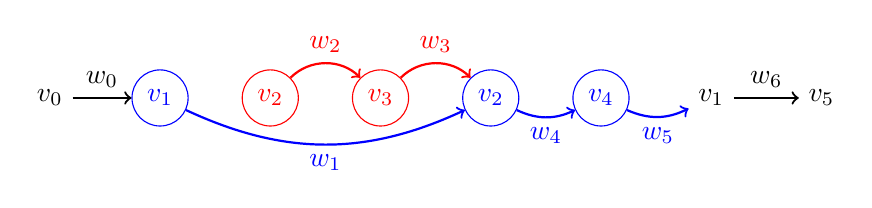
\begin{tikzpicture}
    \tikzstyle{seqc}=[draw, circle]
    \node [] (v0) {$v_0$};
    \node [seqc, blue, right of=v0, node distance=1.4cm] (v1) {$v_1$};
    \node [seqc, red, right of=v1, node distance=1.4cm] (v2) {$v_2$};
    \node [seqc, red, right of=v2, node distance=1.4cm] (v3) {$v_3$};
    \node [seqc, blue, right of=v3, node distance=1.4cm] (v4) {$v_2$};
    \node [seqc, blue, right of=v4, node distance=1.4cm] (v5) {$v_4$};
    \node [right of=v5, node distance=1.4cm] (v6) {$v_1$};
    \node [right of=v6, node distance=1.4cm] (v7) {$v_5$};

    \path[->,thick]
        (v0) edge node [above] {$w_0$} (v1)
        (v6) edge node [above] {$w_6$} (v7)
        ;

    \path[->,thick,bend left=45,red]
        (v2) edge node [above] {$w_2$} (v3)
        (v3) edge node [above] {$w_3$} (v4)
        ;

    \path[->,thick,bend right=25,blue]
        (v1) edge node [below] {$w_1$} (v4)
        (v4) edge node [below] {$w_4$} (v5)
        (v5) edge node [below] {$w_5$} (v6)
        ;
    \end{tikzpicture}

\end{document}